\chapter{Energy Conversion}
\label{ch:conv}

Energy and power take many different forms, from the initial sources to the end results used. Necessarily, methods have been developed to convert the different forms of energy or power from one to another. The first method addressed in this chapter is the conversion process of thermal to mechanical to electrical energy found in heat engines and generators. This thesis is focused on geothermal heat, however heat engines can be used with a number of different sources including the burning of a fuel such as biomass or coal, or even as waste heat from an independent process. Next conversion between different forms of electrical power will be addressed.

%This file used to contain the geothermal chapter, now contains thermal/mechanical section of the conversion chapter
\section{Thermal Energy}
Thermal energy, or heat, can originate from many different sources including combustion of a fuel, radioactive decay, or absorption of light from the sun. Heat can be used directly to warm a building, but it is also a critical step in most traditional methods of generating electrical power. 
%\chapter{Geothermal Energy}
%\label{ch:geothermal}

\subsection{Enthalpy}
Enthalpy describes the energy of a system available to be converted to work. It is related to the temperature of the geothermal resource, but also dependent on the pressure and volume. Temperature is usually the primary metric of a resource, but even a high temperature source is useless without sufficient volume flow. Quantitatively enthalpy is expressed as \cite{Nellis2009}
\begin{equation}
H = U + pV
\end{equation}
where $U$ is the internal energy, which is function of temperature, $p$ is the pressure of the system, and $V$ is the volume. Generally it is more convenient to use the change in enthalpy rather than absolute values. After a system undergoes some thermodynamic process, the system will always have some remaining internal energy, pressure, and volume. Therefore, a change in enthalpy better describes the energy extracted from (or absorbed by) the system.
Additionally, the enthalpy of a system is often normalized by the its mass for comparison to other sized systems and the mass specific enthalpy, $h$, is used instead.
\nomenclature[V]{$H$}{Enthalpy of a fluid\nomunit{\si{\joule}}}
\nomenclature[V]{$U$}{Internal energy of a fluid\nomunit{\si{\joule}}}
\nomenclature[V]{$p$}{Aboluete fluid pressure\nomunit{\si{\pascal}}}
\nomenclature[V]{$V$}{Fluid volume\nomunit{\si{\meter\cubed}}}
\nomenclature[V]{$h$}{Mass specific enthalpy of a fluid\nomunit{\si{\joule\per\kilogram}}}


\subsection{Geothermal Cycles}
%%Describe each of the following but focus on cycles for low enthalpy sources
Geothermal systems can be classified as high-, medium-, or low-enthalpy\footnote{While the technical definitions differ, the terms enthalpy, heat, and temperature are often used interchangeably when qualitatively describing geothermal sources.}. Although there is no formal delineation, high-enthalpy sources generally have temperatures greater than about $150$ \textcelsius{} ($302$ \textdegree{}F) and low-enthalpy sources have temperatures lower than $100$ \textcelsius{} ($212$ \textdegree{}F) \cite{Norden2011}. Depending on the amount of extractable energy of the resource, different geothermal processes or cycles can be used to extract the maximum amount of energy from the resource.

\subsubsection{Dry Steam}
This high-enthalpy processes extracts hot steam from the earth. The steam is sent directly through a turbine then condensed into liquid water and injected back underground. 

\subsubsection{Flash Steam} 
In the flash steam process high pressure hot water is extracted then, allowed to boil becoming steam and low pressure hot water. The steam is sent through a turbine then condensed, recombined with water, and injected back underground.

\subsubsection{Binary Cycle} 
As the name implies, binary cycles involve two loops: a heat source loop and working fluid loop. Heat is collected in the heat source loop and transferred to the working loop through a heat exchanger. The working fluid then undergoes the vaporization process to spin a turbine or other type of expander. The expander is connected to a generator which converts the rotational mechanical energy into electrical energy. After some of the heat is converted, the working fluid passes through a condenser where it is cooled further. Sometimes the cooling process involves drawing in air at ambient temperature, but it can also involve a third loop. The fluids within each of the cycles must be moved using pumps. The pumps themselves need to be powered and act as a parasitic load to the system.

Binary cycles are not limited to low or medium enthalpy heat sources. The most common binary cycle is the Rankine Cycle. A diagram of the process can be seen in \autoref{fig:rankine_cycle_diagram}. In an ideal Rankine Cycle heat is added to the working fluid under high pressure to change its phase from liquid to gas. The fluid expands isentropically\footnote{In thermodynamics, isentropic processes do not have a net change in entropy.} which rotates the generator shaft, causing the fluid's temperature and pressure to drop. Additional heat is then expelled from the fluid as it condenses at a constant low pressure side of the system. Finally the fluid is isentropically pumped back to the high pressure and the process begins again.
\begin{figure}[h]
	\centering

	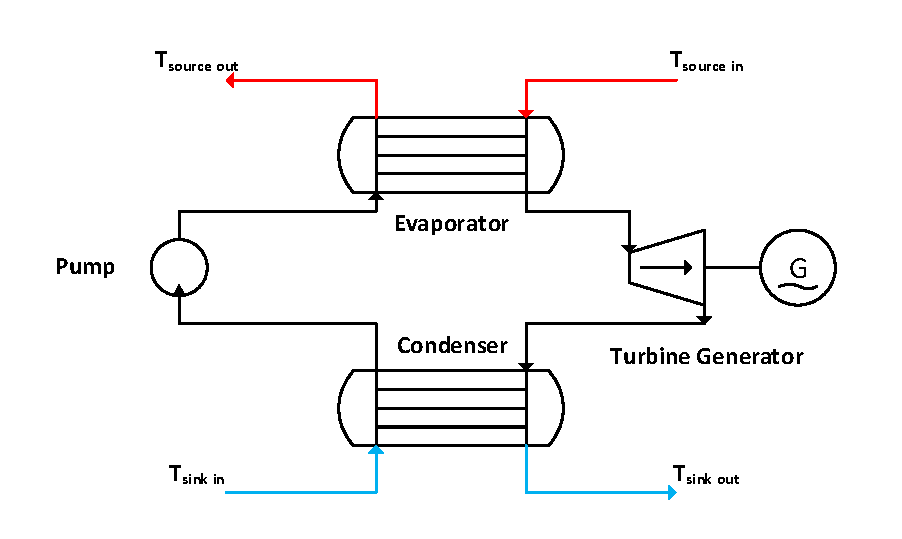
\includegraphics[width=\textwidth]{figures/RankineCycleDiagram.pdf}

	\caption{Diagram of a Rankine cycle system.}
	\label{fig:rankine_cycle_diagram}
	
\end{figure}

For geothermal sources, generally high enthalpy systems can be implemented directly with a single loop using the flash or dry steam processes. However, for lower enthalpy systems, water cannot be used as a working fluid because the temperatures are not high enough to vaporize it. In these cases an organic Rankine cycle, which uses an organic working fluid such as refrigerants instead of water, can be employed. Working fluids are typically selected for relatively low vaporization temperatures, but the thermodynamic states of the heat source must also be considered. The selection of the type of expander and pumps are discussed in Kreider \cite{Kreider}. Generally larger diameter expanders operate at lower speeds.




%\subsection{Pilgrim Hot Springs}
%Do this in 1st chapter not conv/geotherm chapter
%More thourough description of the resource and potential development plans.

 %used to contain geothermal chapter, now contains thermal section

\section{Electric Conversion}

%\subsection{Linear Power Supplies}
%Linear

%\subsection{Switched Mode Power Supplies}

\subsection{PWM vs PFM}

\subsection{DC-DC}
recent developments

\subsection{Rectifiers}
recent developments

\subsection{Inverters}
recent developments
